\begin{htmlonly}
\documentclass{covise}

\usepackage{html, htmllist}
\usepackage{color}
\usepackage{graphicx}
\usepackage{longtable}
\usepackage{palatino}
\usepackage{picins}
\usepackage[colorlinks,dvips]{hyperref}
	  
\bodytext{TEXT=#000000 BGCOLOR=#FFFFFF LINK=#0033CC VLINK=#0033CC}

% #1  mark defined by \label
% #2  a linktext 
% #3  a html link 
\newenvironment{covlink}[3]%
{\html{\htmladdnormallink{#1}{#3}}\latex{\hyperref[#1]{#2} (\ref{#1})}%
}

\newenvironment{covimg}[4]%
{ \html{\htmladdimg[ALIGN=CENTER]{#2.gif}}
 
 \latexonly
 \begin{figure}[!Hhtp]
  \begin{center}
   \includegraphics[scale=#4]{#1/#2}
   \caption{#3}
  \end{center}
 \end{figure}
 \endlatexonly
}



\definecolor{output}{rgb}{0.,0.,1.}
\definecolor{depend}{rgb}{1.,0.65,0.}
\definecolor{required}{rgb}{0.58,0.,0.83}
\definecolor{optional}{rgb}{0.,0.39,0.}

\end{htmlonly}

%================================================================================
%================================================================================
%
%   
%================================================================================
%\startdocument

\chapter{Usage}

\section{Start Screen - How to use COVER}

This chapter familiarizes you with the Virtual Reality interface to execute the process steps described in
detail in chapter 2.\newline 

The process steps are

\begin{enumerate}
\item Select {\bf Sheet Size}
\item Define {\bf Knob Shape}
\item {\bf Pattern Design}
\item {\bf Embossing}
\item Presentation as {\bf Roll} or {\bf Sheet} 
\item {\bf Traction Sim} (Traction Simulation]
\end{enumerate} 

Select the steps in the specified order - otherwise you will get warnings!  
\newline
\newline
In addition, you get
\newline 
\begin{figure}[!Hhtp]
%  \begin{center}
   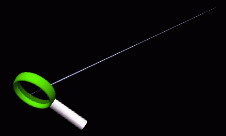
\includegraphics[scale=1.0]{usage/scale}
%  \caption{Scale}
%  \end{center}
\end{figure} \newline
and {\bf View All}\newline \newline
to scale the output.

\begin{figure}[!Hhtp]
  \begin{center}
   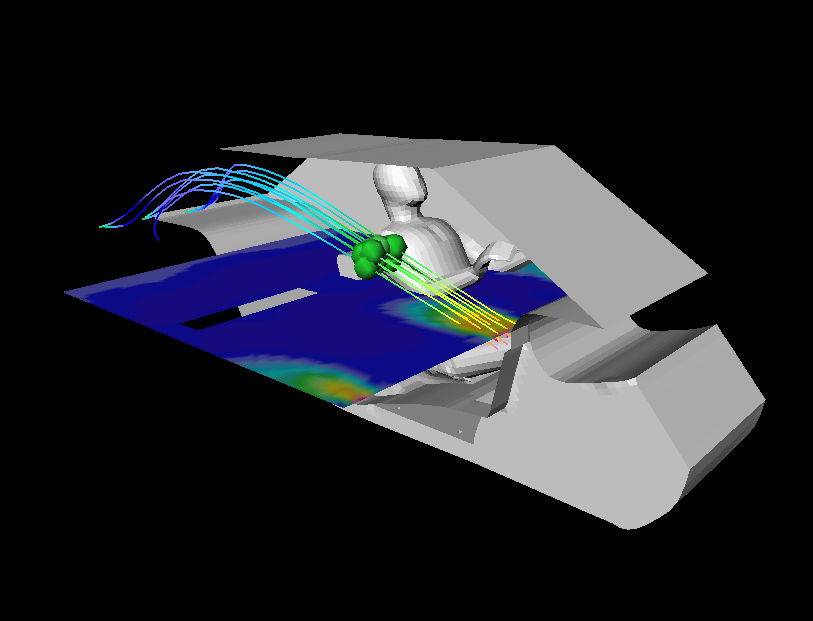
\includegraphics[scale=0.4]{usage/start}
   \caption{Start Screen}
  \end{center}
\end{figure}


%--------------------------------------------------------------------------

{\bf How to use COVER}\newline
\newline
The VR interface for the SCA E-Type Project is implemented using COVER. COVER (COvise Virtual Environment Renderer) is a COVISE renderer module
with support for Virtual Reality (VR) input devices, backprojection displays,
and intuitive interaction. Below some basic information about working with COVER
is provided.

In COVER the user can freely move in the virtual scene  
and manipulate it with a {\bf 3D input device}.\newline
\newline
The movement of the user is measured with a sensor 
mounted at the glasses. With the measured position and orientation an 
appropriate view on the scene is computed. This is called {\bf head tracking}.
Currently only one user can be tracked. Other users don't have the correct 
view of the scene and therefore they have the impression that all objects 
are slightly distorted. This effect is minimized if they try to stand close 
to the user with the tracked glasses and try to look into the same 
direction as the one with the tracked glasses.\newline 
\newline
The location and orientation of the 3D input device, which the user
holds in his hand, is measured through a sensor in the input device.
The input device usually has one two three buttons. One button is 
used to indicate a selection. On a three button device the other two buttons
are used to switch the navigation mode without using the 3D menu.\newline
\newline
With the {\bf virtual laser beam} which seems to come out of the 3D input device also
remote objects can be reached, for example buttons in the 3D menu.\newline
\newline
%COVER can also be used with the {\bf mouse}.\newline
%\newline
%The navigation mode, viewing options, and manipulation modes are
%selected through a 3D menue, called the Pinboard. 
You select a menu entry
by pointing to the button with the laser beam and pressing the 
button of the 3D input device. 
%If the pinboard is used with a mouse
%simply bring the mouse pointer over the menu entry and click a button.\newline
%\newline
A menu can be re-positioned in the Virtual Environment by pointing to the title bar
and pressing the button of the 3D input device. If you have a 3-button device
and select it the left button, the menu is rotated around it's z axis so it 
always faces the viewer (billboard mode). Selected with the right button, it moves as if it's
mounted at the laser beam. Selected with the middle button
it changes it's size according to the rotation of the users arm.\newline 
\clearpage
%The same applies for mouse input: left mouse button moves the menu in a 
%way that it faces the viewer, right mouse button moves the menu with the
%mouse pointer. The orientation is defined through a line from the viewer
%to the mouse so it seems to face the viewer, too. Middle mouse button
%scales the menu, movements up and down make the menu larger and smaller. 
In {\bf XFORM (Transform) mode} the whole scene 
%(besides the coordinate axis and the pinboard) 
can be moved. 
%The default button label is "move world" and
%the default button location is in the main Pinboard menue. 
%The XFORM mode indicated with the above 3D icon.\newline
\newline
XFORM mode is on the right button.
Only when the button of the 3D input device is pressed, the world
is translated and rotated with the users hand. The translation is relative 
to the point where the button was pressed. The center of rotation is the users
hand. The interaction is stopped when the button is released. For pulling
the whole scene closer to the user you can move the hand away from the body, 
then press the button and move the hand closer too the body, and then relase 
the button. Do this several times if the appropriate position can't be 
reached in one step.\newline 
\newline
%If the input device is the mouse, the scene is rotated when the left
%mouse button is pressed and translated when the middle mouse button
%is pressed. In rotate mode, up/down movements rotate around the x axis, 
%left/right movements rotate around the z axis. In translate mode, up/down
%movements translate into positive and negative z direction, left/right movements 
%into positive/negative x axis.\newline
%\newline
\begin{figure}[!Hhtp]
  \begin{center}
   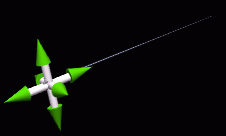
\includegraphics[scale=1.0]{usage/xform}
   \caption{XFORM (Transform = Move World) Mode Icon}
  \end{center}
\end{figure}
For more information about COVER see COVISE User's Guide, chapter COVER, section Interaction.
%--------------------------------------------------------------------------
\clearpage

\section{Sheet Size}

This process step allows you the selection of the following sheet sizes:

\begin{itemize}
\item 3 standard sizes of toilet paper
	\begin{itemize}
   	\item Toipa 125x98 [mm] 
  	\item Toipa 140x98 [mm]
	\item Toipa 125x110 [mm]
	\end{itemize}
\item 2 standard sizes of household paper	
	\begin{itemize}
   	\item HHT 246x260 [mm]
  	\item HHT 246x230 [mm]
	\end{itemize}
\item Custom Dimensions (select your own size - for range of allowable values see table in chapter 2)
	\begin{itemize}
   	\item variable length [mm]
  	\item variable width [mm]
	\end{itemize}
\end{itemize}

\begin{figure}[!Hhtp]
  \begin{center}
   \includegraphics[scale=0.4]{usage/sheet_size}
   \caption{Sheet Size}
  \end{center}
\end{figure}
\clearpage

\section{Knob Shape}

This process step allows you to 
\begin{itemize}
\item select the basic {\bf Knob Shape} (choice)
	\begin{itemize}
	\item {\bf Circle}	
	\item {\bf Ellipse}
	\item {\bf Rectangle}
	\end{itemize}
\item specify the size of the knob (for range of allowable values see table in chapter
2)
	\begin{itemize}
	\item {\bf Length [mm]} 
	\item {\bf Width [mm]} (Length=Width=Diameter in cas of circle)
	\item {\bf Height [mm]} 
	\item {\bf Flank Angle [$\symbol{23}$]} (should be '$\symbol{23}$' instead of 'mm' in figure below)
	\end{itemize}	
\item specify the 'smoothing of the edges' (for range of allowable values see table in chapter
2)
	\begin{itemize}
	\item {\bf Abrasion Radius [mm]}
	\item {\bf Ground Radius [mm]}
	\end{itemize}
\item compare with a {\bf DataBase} (choice)
	\begin{itemize}
 	\item use values as parameters for a new knob 
	(and start time-consuming simulation later on) 
	\item look if same or similar knob is already in database
	(and use the results to avoid another simulation run)
	\end{itemize}	
\end{itemize}


\begin{figure}[!Hhtp]
  \begin{center}
   \includegraphics[scale=0.4]{usage/knob_shape}
   \caption{Knob Shape}
  \end{center}
\end{figure}
\clearpage

\section{Design}

There are two options for Pattern Design:
\begin{itemize}
\item {\bf Parametric Design}:\newline
 In this case you specify a couple of parameters
 	\begin{itemize}
	\item {\bf Angle} [$\symbol{23}$] 
	\item {\bf Distance} [mm]
	\end{itemize}
For the meaning of these parameters and the range of allowable values see chapter 2!
The complete pattern is generated by replicating the repeating pattern.
	
\item {\bf Free Design}:\newline 
In this case you read the positions of the knobs from a file.
This file contains the size of the repeating pattern  
	\begin{itemize}
	\item {\bf Rapport Length} [mm] 
	\item {\bf Rapport Width} [mm]
	\end{itemize}
You can see and change these values in the Free Design menu. \newline
Please note: The menu (COVER) allows you to specify
values in the range given by the COVISE map. To extend this range you have to
use the map (see chapter 3.10 - ControlSCA module).\newline
  
In addition, this file contains 
	\begin{itemize}
	\item the {\bf number of knobs} and 
	\item the {\bf coordinates of the knobs} relative to
	the bottom left corner of the repeating pattern. 
	\end{itemize}
You see a representation of these knobs in the upper right section of the 
Free Design window (see figure 'Design') and you can interactively 
	\begin{itemize}
	\item {\bf move a knob} (shown in red):\newline
	Select knob with laser beam, press button, keep it pressed and move knob by moving
	your 3D-input device
	\item {\bf destroy a knob}:\newline
	Select knob with laser beam, press button, keep it pressed 
	and {\bf move knob out of the repeating pattern}by moving
	your 3D-input device 
	\item {\bf add a new knob}:\newline
	Point with the laser beam to a position in the rapport, click 
	- new knob appears 
	\end{itemize}
The move operations are checked:	 
	\begin{itemize}
	\item As long as you don't get too close to another knob 
	all knobs are encircled \newline 
        {\bf blue (= legal operation)}, see figure 'Design'. 
	\item If you get too close to another knob both knobs are encircled \newline 
	{\bf yellow (= design check)}, see figure 'Design Check'. 
        \end{itemize}
\end{itemize} 

\begin{figure}[!Hhtp]
  \begin{center}
   \includegraphics[scale=0.4]{usage/design}
   \caption{Design}
  \end{center}
\end{figure}

\begin{figure}[!Hhtp]
  \begin{center}
   \includegraphics[scale=0.4]{usage/design_check}
   \caption{Design Check}
  \end{center}
\end{figure}
\clearpage

\section{Embossing}

The menu item provides options for simulating the embossing (or to skip it if results for same
or similar options are already available). The user may 

\begin{itemize} 
\item set parameters
	\begin{itemize}
	\item {\bf Rubber Hardness [Shore]}   
	\item {\bf Contact Pressure [N/cm2]}
	\item {\bf Tissue Type:}
		\begin{itemize}
		\item TAD
		\item Slush
		\item Double Velvet
		\item HHT Convent
		\item HHT
		\item BSQ A
		\end{itemize}
	\end{itemize} 		 
\item and decide to 
	\begin{itemize}
	\item {\bf Start Embossing} or  
	\item look at the {\bf Database} first
	\end{itemize}
\end{itemize}

Please note:

\begin{itemize}

\item Currently the value for Rubber Hardness is ignored (except that it is stored in the database), 
and simulation starts with predefined values.

\item Contact Pressure actually meens the maximum force applied {\bf per knob}. This value
can be modified within a range defined in the map. The values in the map may have to be
adjusted if sufficient experience has been gained with this model.
 
\item Searching the data base means: first, search for the same material, 
second, list all knobs that differ in hardness of rubber and contact pressure 
not more than 10 \%.
\item The simulation of embossing is carried out by using LS-Dyna and may take a
considerable amount of time, depending on the computer you are running on. So it may be
worth to use 'similar' results, if possible.

\end{itemize}
	
\begin{figure}[!Hhtp]
  \begin{center}
   \includegraphics[scale=0.4]{usage/embossing}
   \caption{Embossing}
  \end{center}
\end{figure}
\clearpage

\section{Meshing/Photorealistic Representation}

All grids of the embossed knobs within the repeating pattern are combined into an overall
grid using the Ansys program. This step is transparent ot the user - no visible result,
but it takes a few minutes.
After meshing a photorealistic impression is achieved by superimposing a texture on the
deformed grid. If you look at the Fig. 'Meshing' below, you see that you have a choice for
the 
{\bf Presentation}
\begin{itemize}
\item {\bf Roll}
\item {\bf Sheet}
\end{itemize} 

You see the results in the figures 
\begin{itemize}
\item Presentation: Roll
\item Presentation: Sheet
\end{itemize} 
 

\begin{figure}[!Hhtp]
  \begin{center}
   \includegraphics[scale=0.4]{usage/meshing}
   \caption{Meshing}
  \end{center}
\end{figure}
\clearpage

\section{Presentation as Roll or Sheet}

\begin{figure}[!Hhtp]
  \begin{center}
   \includegraphics[scale=0.4]{usage/presentation_roll}
   \caption{Presentation: Roll}
  \end{center}
\end{figure}

\begin{figure}[!Hhtp]
  \begin{center}
   \includegraphics[scale=0.4]{usage/presentation_sheet}
   \caption{Presentation:Sheet}
  \end{center}
\end{figure}
\clearpage

\section{Traction Simulation}

The simulation of the traction test calculates a measure for the deformation within {\bf one rapport}.
To be more accurate: The current implementation calculates the von-Mises stress for the
grid cells. This is a measure for the inhomogenity of forces applied to the grid cell: The
higher the value the more likely the paper will tear at that point.
\newline
\newline
The {\bf Traction} menu item provides options to
\begin{itemize}
\item {\bf Start Traction}: Start Traction Simulation
\item {\bf Colors}: Show color legend for deformation of the grid cells
\end{itemize}

\begin{figure}[!Hhtp]
  \begin{center}
   \includegraphics[scale=0.4]{usage/traction_start}
   \caption{Traction Start}
  \end{center}
\end{figure}

\begin{figure}[!Hhtp]
  \begin{center}
   \includegraphics[scale=0.4]{usage/traction_results}
   \caption{Traction Results}
  \end{center}
\end{figure}
\clearpage



\section{Scale World/View All}

\begin{figure}[!Hhtp]
%  \begin{center}
   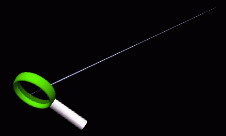
\includegraphics[scale=1.0]{usage/scale}
%  \caption{Scale}
%  \end{center}
\end{figure}

In SCALE mode the whole scene can be scaled. 
When the button of the 3D input device is pressed and the hand is
moved to he right, the world becomes larger, when the hand is moved
to the left, the world becomes smaller. The interaction is stopped when the
button is released.
The same applies for mouse input.
 		
{\bf View All}

When the VIEW ALL button is pressed, the whole scene is scaled so that it fits into 
the visible part of the world - typically the screen size. 
\clearpage

\section{Map - Info only!}

Below you see the COVISE map used for the complete process. If everything works fine
you don't need the map - it's for information only. In case of errors, however, the
map may be useful for localizing and describing a problem.


\begin{figure}[!Hhtp]
  \begin{center}
   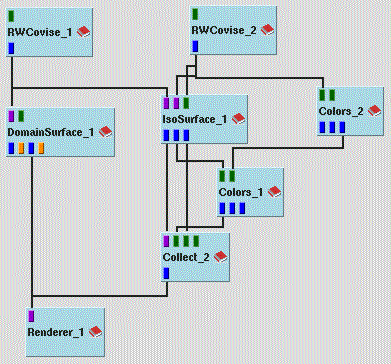
\includegraphics[scale=0.4]{usage/map}
   \caption{Map}
  \end{center}
\end{figure}
\clearpage
